\section{Detalii despre dezvoltarea aplicației}

	Dezvoltarea a început cu prima întâlnire între conducerea companiei, utilizatori și mine, unde s-au stabilit modulele aplicației:
	\begin{enumerate}
		\item Înregistrarea daunelor:
		\begin{enumerate}
			\item Înregistrarea cererii de despăgubire online.
			\item Atașarea evidențelor -- poze sau alte documente justificative.
		\end{enumerate}
		\item Introducerea datelor vânzărilor săptămânale (import).
		\item Sistemul de decizii:
		\begin{enumerate}
			\item Asocierea cererii de despăgubire cu contractul de asigurare întocmit la achiziția produsului.
			\item Luarea deciziei de reparație sau înlocuire.
			\item Actualizarea evoluției deciziei din punctul de vedere și al costului soluționării cererii de despăgubire.
		\end{enumerate}
		\item Sistemul de raportare:
		\begin{enumerate}
			\item Statistici rapide (câte cereri de despăgubire, decizii au fost create în perioada respectivă de timp).
			\item Raport cu toate deciziile plătite într-o anumită perioadă de timp.
			\item Raport cu numărul de asigurări, grupate în funcție de tipul de asigurare și prețul ei, în perioada respectivă.
			\item Raport cu numărul vânzărilor asigurărilor grupate în funcție de magazinul ce a făcut vânzarea, împreună cu perioada când s-a vândut primul și ultimul produs.
			\item Raport detaliat despre produsele ce încă sunt asigurate, împreună cu posibila cerere de despăgubire asociată.
		\end{enumerate}
	\end{enumerate}

	Accentul s-a pus pe dorința de a scoate rapoarte, unitare și flexibile, și micșorarea numărului de fișiere accesate.

	Pe tot parcursul dezvoltării aplicației, am fost singurul decident și dezvoltator, referitor la:
	\begin{itemize}
		\item Arhitectura aplicației informatice.
		\item Construirea bazei de date.
		\item Împărțirea aplicației în module interconectate și flexibile.
		\item Migrarea spre o soluție de găzduire partajată.
		\item Securitatea datelor.
		\item Interacțiunea utilizatorilor și a clienților cu aplicația.
		\item Soluții și strategii de backup.
	\end{itemize}

	Pe parcursul dezvoltării în mediul de test, rigiditatea legăturilor dintre module, impusă inițial, a fost întâmpinată cu rezistență, din cauza libertății oferite de Excel, dar exactitatea rapoartelor obținute au fost în favoarea soluției adoptate.

	Interacțiunea cu clientul a fost gândită a fi cât mai rapidă și eficace.
	Atunci când intră pe pagina aplicației, el poate deja să completeze cererea de despăgubire, așa cum se poate observa în figura~\ref{fig:pagina_principala}.
	Clientul este îndrumat pentru a completa cât mai detaliat detaliile despre cererea de despăgubire și este avertizat atunci când apare o eroare sau a uitat să completeze un câmp necesar.
	\begin{figure}
	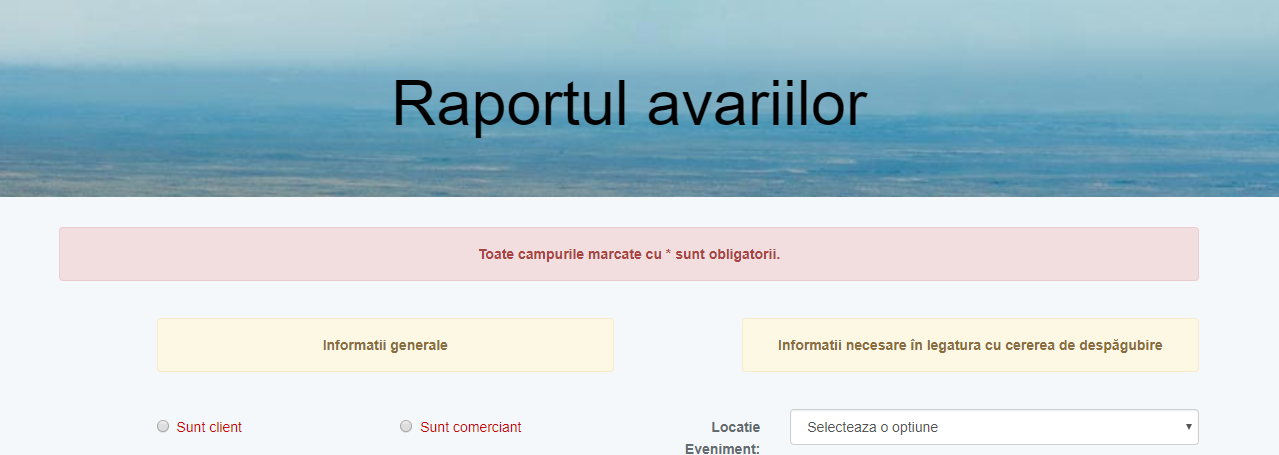
\includegraphics[width=\linewidth]{../imagini/main.png}
	\caption{Pagina principală a \url{https://fandu.info}}
	\label{fig:pagina_principala}
	\end{figure}

	Am ales să implementez baza de date și codul aplicației la o companie de încredere ce oferă soluții de găzduire partajată \url{https://xServers.ro}\cite{xservers}.
	Dar pozele și spațiul de stocare a pdf-urilor încărcate de client sunt găzduite de Amazon Web Services\cite{aws}, pentru a beneficia de prețul redus și valabilitatea extinsă a fișierelor pe „cloud”.
	Avantajul soluției alese este traficul de internet necontorizat și spațiu de stocare suficient.

	De asemenea, au fost implementate sisteme de backup săptămânal a bazei de date, arhivate și encriptate în a terța locație.

	Codul sursă este ținut într-un proiect „git”, un sistem de gestionare și versionare a codului de programare, încărcat și protejat pe GitHub.
